\documentclass[tikz,border=2mm]{standalone}
\usetikzlibrary{shapes.geometric, arrows, positioning}
\begin{document}
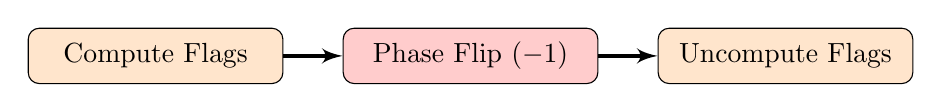
\begin{tikzpicture}[
    node distance=3cm,
    block/.style={rectangle, draw, fill=orange!20, text width=3cm, text centered, rounded corners, minimum height=2em},
    line/.style={draw, -latex', ultra thick}
]

\node [block] (compute) {Compute Flags};
\node [block, fill=red!20, right of=compute, node distance=4cm] (phase) {Phase Flip ($-1$)};
\node [block, right of=phase, node distance=4cm] (uncompute) {Uncompute Flags};

\path [line] (compute) -- (phase);
\path [line] (phase) -- (uncompute);

\end{tikzpicture}
\end{document}
